% Figura Anexo I: qué es una rigidez real: el precio deseado apenas responde a la demanda y el coste de menú muerde
\documentclass[tikz,border=3pt]{standalone}
\usepackage[T1]{fontenc}
\usepackage[utf8]{inputenc}
\usepackage{amsmath}
\usetikzlibrary{arrows.meta,calc,positioning}
\begin{document}
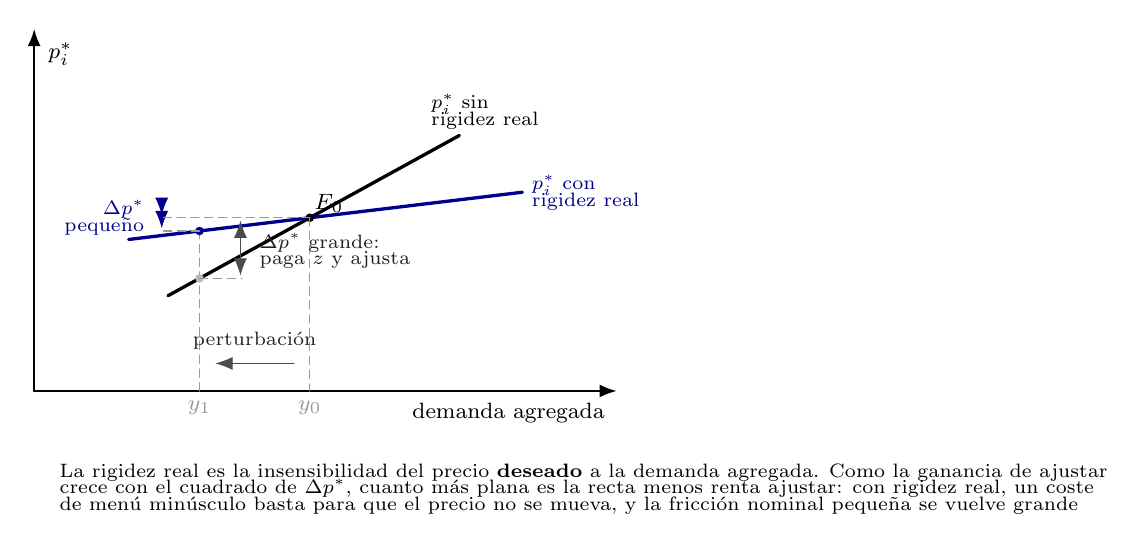
\begin{tikzpicture}[>={Latex[length=2.2mm]}, line cap=round, font=\footnotesize,
  eje/.style={->, thick},
  curva/.style={very thick},
  nueva/.style={very thick, blue!55!black},
  guia/.style={densely dashed, gray!80},
  pto/.style={circle, fill=black, inner sep=1.1pt}]
  \draw[eje] (0,0) -- (7.4,0) node[below left=1pt]{demanda agregada};
  \draw[eje] (0,0) -- (0,4.6) node[below right=2pt]{$p^{*}_{i}$};
  % Sin rigidez real: pendiente fuerte
  \draw[curva] (1.7,1.21) -- (5.4,3.245);
  \node[anchor=west, inner sep=1pt, align=left, font=\scriptsize] at (5.0,3.55) {$p^{*}_{i}$ sin\\[-2pt]rigidez real};
  % Con rigidez real: casi plana
  \draw[nueva] (1.2,1.924) -- (6.2,2.524);
  \node[anchor=west, inner sep=1pt, blue!55!black, align=left, font=\scriptsize] at (6.28,2.52) {$p^{*}_{i}$ con\\[-2pt]rigidez real};
  % Punto inicial y shock
  \node[pto] (E0) at (3.5,2.2) {};
  \node[above right=-1pt of E0, inner sep=1pt] {$E_0$};
  \draw[guia] (3.5,2.2) -- (3.5,0) node[below]{$y_0$};
  \draw[guia] (2.1,0) node[below]{$y_1$} -- (2.1,2.032);
  \node[pto, fill=blue!55!black] (Ar) at (2.1,2.032) {};
  \node[pto, fill=gray!55] (An) at (2.1,1.43) {};
  \draw[->, gray!60!black] (3.3,0.35) -- (2.3,0.35);
  \node[font=\scriptsize, anchor=south, text=gray!25!black] at (2.8,0.4) {perturbación};
  % Brechas de precio deseado
  \draw[<->, blue!55!black, shorten >=1pt, shorten <=1pt] (1.62,2.2) -- (1.62,2.032);
  \node[anchor=east, font=\scriptsize, blue!55!black, align=right] at (1.52,2.2) {$\Delta p^{*}$\\[-2pt]pequeño};
  \draw[guia] (2.1,2.032) -- (1.64,2.032);
  \draw[guia] (3.5,2.2) -- (1.64,2.2);
  \draw[<->, gray!60!black, shorten >=1pt, shorten <=1pt] (2.62,2.2) -- (2.62,1.43);
  \node[anchor=west, font=\scriptsize, gray!25!black, align=left] at (2.74,1.78) {$\Delta p^{*}$ grande:\\[-2pt]paga $z$ y ajusta};
  \draw[guia] (2.1,1.43) -- (2.64,1.43);
  \node[align=left, anchor=north west, font=\scriptsize] at (0.2,-0.8)
    {La rigidez real es la insensibilidad del precio \textbf{deseado} a la demanda agregada. Como la ganancia de ajustar\\[-2pt]crece con el cuadrado de $\Delta p^{*}$, cuanto más plana es la recta menos renta ajustar: con rigidez real, un coste\\[-2pt]de menú minúsculo basta para que el precio no se mueva, y la fricción nominal pequeña se vuelve grande};
\end{tikzpicture}
\end{document}
